\documentclass[12pt]{article}
\usepackage[a4paper, left=2cm, right=2cm, top=2cm, bottom=2cm]{geometry}
\usepackage[utf8]{inputenc}
\usepackage[T1]{fontenc}
\usepackage[french]{babel}
\usepackage{graphicx}
\usepackage{lmodern}
\usepackage{csquotes}
\usepackage[backend=biber,style=numeric,sorting=none]{biblatex}
\usepackage[xindy]{glossaries}
\usepackage[hidelinks]{hyperref}
%\graphicspath{ {images/} }
 
\parskip=5pt plus2pt minus 1pt
\frenchbsetup{ReduceListSpacing=false}

\catcode`\|=13
\def|#1|{\texttt{\detokenize{#1}}}

\addbibresource{bibli.bib}
\makeglossaries

\title{\gls{PdP} \smallbreak Mémoire }
\author{Lorian Corbel \\ Camille Meyrignac \\ Maxime Pacaud \\ Nicolas Sentout}

\begin{document}

% ACRONYMS HERE
\newacronym{PdP}{PdP}{Projet de Programmation}
\newacronym{GPU}{GPU}{Graphics Processing Unit}
\newacronym{GLSL}{GLSL}{OpenGL Shading Language}
\newacronym{VBO}{VBO}{Vertex Buffer Object}
\newacronym{IBO}{IBO}{Index Buffer Object}
\newacronym{VAO}{VAO}{Vertex Array Object}

% DEFINITIONS HERE
\newglossaryentry{marque}
{ 
    name=marque,  
    description={Les marques sont les éléments basiques, c'est à dire des formes primitives dont les
    propriétés peuvent être gérées par des données liées} 
}
\newglossaryentry{canaux}
{ 
    name=canaux,  
    description={Caractéristique d'une marque; ex: position, taille, rotation, profondeur, couleur, etc} 
}
\newglossaryentry{crate}
{
    name=crate,  
    description={Une crate est une collection de code source Rust} 
}
\newglossaryentry{shader}
{
    name=shader,
    description={Programme GLSL}
}
\newglossaryentry{vertex}
{
    name=vertex,
    description={Point d'informations graphiques}
}
\newglossaryentry{uniform}
{
    name=uniform,
    description={Un uniform est une variable globale GLSL}
}
\newglossaryentry{pipeline}
{
    name=pipeline,
    description={Succession des opérations généralement réalisées par une carte graphique nécessaires au
    rendu d'un lot de données}
}
\newglossaryentry{geom}
{
    name={geometry shader},
    description={Un programme shader écrit en GLSL qui régit le traitement des primitives (marque)}
}

\newglossaryentry{unsafe}
{
    name={unsafe},
    description={Partie de code qui ne garantit pas la sécurité de mémoire promis par Rust}
}

\maketitle
\tableofcontents
\newpage

\section{Abstract}

De nos jours le Big Data demande de créer des bibliothèques de visualisation de données pouvant afficher plusieurs centaines de milliers de visuels tant en maintenant un nombre d'image par seconde satisfaisant. 
C'est dans ce contexte qui nous a été demandé de réaliser un moteur de rendu en Rust gérant les animations et dont la performance est l'objectif principal. Nous avons réalisé une bibliothèque pouvant manipuler plusieurs types de formes, supportant les animations et dont les performances sont supérieurs à celles de bibliothèques similaires.  
 

\section{Travaux précédents}

Nous nous sommes basés sur deux bibliothèques afin de réaliser ce projet.
Premièrement la bibliothèque FATuM, une bibliothèque C++ qui se veux être un compromis entre le heut et le bas niveau, la bibliothèques donne la possibilité d'autres bibliothèques dont l'interface serait plus adapté pour une utilisation de haut niveau sans avoir à ce soucier de la vitesse de rendu.

La seconde bibliothèques, vega écrite en javascript est une bibliothèque visant à donner divers outils de dessin pour des bibliothèques de plus haut niveau.

Finalement notre client nous a aussi donner un proof of concept de ce que nous devions implémenter. Écrite en Rust, cette bibliothèque propose l'affichage de plusieurs type de forme que nous devions nous aussi être capable d'afficher.    

\section{Analyse des besoins}
%% Etoffer la partie analyse des besoins
\section{Analyse des besoins fonctionnels}

L'utilisateur doit être capable d'appeler des fonctions de la bibliothèque permettant d'afficher des
\gls{marque}s \cite{VegaMarks}. Il doit notamment être capable de préciser des \gls{canaux} associés à
ces marques : la position de la marque, sa taille, sa rotation, sa profondeur, sa couleur, sa forme,
l'épaisseur et la couleur de son contour, son contraste, sa luminance, son rayon, ses angles, etc.
\textit{Contrast} offrira la possibilité d'afficher les marques suivantes : 
\begin{itemize}
    \item Points : utilisable pour faire des nuages de points. La forme des points dépend d'une fonction de
    distance calculée en GLSL. Les marques de type Points peuvent prendre différentes formes (triangle, rectangle, diamant, trèfle, astérisque, etc.).
    \item Lignes : utilisable tel quel ou pour faire des connexions entre d'autres marques. Les lignes
    peuvent être des segments, des polylignes ou des courbes, elles peuvent aussi avoir différents types
    (continu, tirets, pointillés...).
    \item Polygones : utilisable pour représenter des polygones pleins ou vides, où l'on appelle vide un 
    polygone dont seulement les contours sont dessinés, la couleur de remplissage du polygone plein peut être
    différente de la couleur des contours.
    \item Aires : utilisable pour représenter des polygones ayant un mode d'affichage légèrement différent
    \cite{VegaMarks}.
    \item Texte : utilisable pour représenter du texte et peut avoir différentes propriétés : italique,
    gras, centré, aligné à droite, en haut, etc.
\end{itemize}
    
Pour tester cette fonctionnalité, il devra y avoir des tests permettant d'afficher des marques de façon
contrôlée et de ce fait vérifier si les marques s'affichent bien suivant leurs \gls{canaux} associés.

\textit{Contrast} devra également être capable de gérer des calques, c'est-à-dire que l'utilisateur pourra
décider de placer une marque sur un certain calque et une autre marque sur un différent calque. Si ces
marques ont la même position, l'une des deux marques cachera la seconde. Cet exemple utilise deux calques
mais il peut y en avoir autant que l'utilisateur le souhaite.

Une caméra simple pour visualiser la scène en 2D doit être implémentée. À priori, elle ne fait pas
de translation, le seul paramètre qu'elle prend en compte est un niveau de zoom ainsi que la taille
de la fenêtre d'affichage.

Ces marques pourront également être animées. La gestion des animations sera implémentée de manière similaire
à FATuM, c'est-à-dire avec un double tampon pour la visualisation, un tampon servant de tampon avant et un tampon servant de tampon arrière. Le tampon avant est utilisé pour l'affichage et le tampon arrière est utilisé pour les modifications de l'image affichée et quand l'opération de mise à jour est finie (c'est-à-dire que l'on a une autre image à afficher). Les deux tampons peuvent être échangés par différentes techniques notamment un simple échange : le tampon arrière devient le tampon avant et inversement, ou on peut utiliser une interpolation progressive des deux images stockées dans les tampons. De ce fait, l'image affichée n'est changée que quand il y a une autre image prête, ce qui évite le problème de l'affichage se mettant à jour petit à petit, donnant lieu à des animations peu lisible. Un troisième tampon peut être utilisé pour empêcher l'annulation d'une animation si l'utilisateur demande une modification pendant une animation. Le troisième tampon stocke les modifications faites par l'utilisateur durant l'animation et seront utilisées pour la prochaine animation.

Dans un premier temps la bibliothèque ainsi développée devra être capable d'afficher,
à 50 images par seconde, au moins 10 fois plus d’éléments que la librairie JavaScript D3.js. 
Le but final étant que \textit{contrast} ait de meilleures performances que FATuM.

\section{Analyse des besoins non fonctionnels}

Selon le client, il serait préférable d'implémenter les marques dans l'ordre suivant :
\begin{itemize}
    \item Points
    \item Lignes
    \item Polygones
    \item Aires
    \item Texte
\end{itemize}

Concernant l'API de \textit{contrast}, l'utilisateur n'aura pas accès aux
couches inférieures à la bibliothèque. Il n'aura pas accès aux types des marques,
il décrira seulement les propriétés de la marque et \textit{contrast} déterminera
s'il s'agit d'une marque de type point, ligne, texte, etc.
Voici un exemple de syntaxe pour ajouter une marque de type Texte :

|addMark().set_center(0.5,0.5).set_color(Color.Blue)|\newline
|.set_font("ComicSansMS").set_font_size(20).text("Bonjour").show()|

Notons que cette syntaxe n'est pas définitive mais cela donne une idée de la façon
dont l'utilisateur manipule les marques.

Notre client souhaite que nous utilisons une crate Rust pour compiler
nos shaders en GLSL, afin de construire et nous assurer de leur bonne conformité.
La crate en question porte le même nom que GLSL\cite{GLSL}.

Pour atteindre les demandes de performances imposées par le client, nous allouerons les données au maximum possible sur la pile.
La consommation mémoire n'est pas une contrainte importante pour le développement de \textit{contrast}. Tant
que la vitesse est satisfaisante, nous n'aurons pas à optimiser au mieux la gestion de la mémoire.

Nous devrons mettre en place une batterie de tests importants car ce genre de bibliothèque impose de faire
du code \og non stable \fg{}.
C'est-à-dire du code qui désactive les garanties de sécurité comme celle citée dans l'introduction.
Ces tests permettront en outre de valider nos structures de données.
Nous allons également réaliser des tests de performance afin de nous assurer que notre solution réponde bien
aux exigences de vitesse qui nous sont fixés.

\section{Description du logiciel}
%% Parler des problèmes rencontrés au sain de l'archi
%% Remplacer cette archi outdated
\subsection{Description de l'architecture}

Ce diagramme, disponible ici (figure~\ref{fig:arch}), décrit les structures, énumérations et traits
(interfaces) qui seront utilisés dans le projet. Il n'y a ni classes, ni héritage dans Rust. C'est
pourquoi ce diagramme est différent d'un diagramme de classes classique.

\begin{figure}[htp]
  \centering
  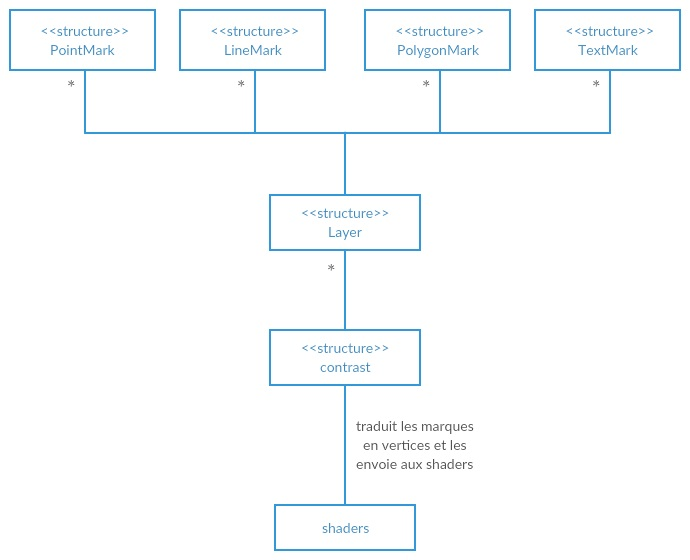
\includegraphics[scale=0.35]{images/architecture}
  \caption{Diagramme de l'architecture de \textit{contrast}}
  \label{fig:arch}
\end{figure}

\subsection{Schéma du pipeline}

Cette figure~\ref{fig:pipe} présente la décomposition des différents éléments nécessaire au \gls{pipeline}
graphique pour chaque marque. Le pipeline peut être externe à notre bibliothèque, il doit juste demander
les canaux, autrement dit les vertices (\gls{vertex}), contenu dans le \gls{VBO} et les \gls{uniform}
du \gls{shader} à notre bibliothèque\cite{Semi}.
Dans notre cas, c'est \textit{luminance} qui est en charge du pipeline.

Le renderer n'est actuellement pas présent dans notre diagramme de l'architecture pour des 
raisons techniques. Son rôle est d'indexer les marques de chaque type. Quand une marque demande
à être affiché, elle notifie le renderer qui va récupérer ses canaux et construire le VBO.




\begin{figure}[htp]
  \centering
  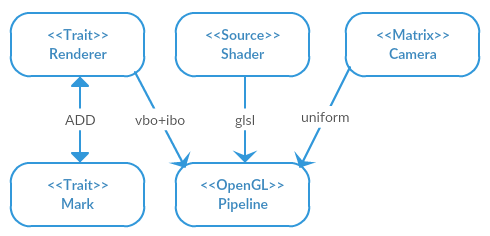
\includegraphics[scale=0.8]{images/pipeline}
  \caption{Diagramme de schématisation du pipeline}
  \label{fig:pipe}
\end{figure}

%% Parler des problèmes rencontrés au sain de l'archi

\subsection{Imlémentation des marques point}

\subsection{Implémentation des marques ligne}

\subsection{Implémentation des marques texte}

\subsection{Les calques}
\subsubsection{Qu'est-ce qu'un calque ?}
Un calque est un groupe de marques ayant en commun une profondeur. C'est-à-dire que les marques étant dans
un calque de profondeur 0 apparaîtront devant des marques appartenant à un calque de profondeur 1.

\begin{figure}[htp]
  \centering
  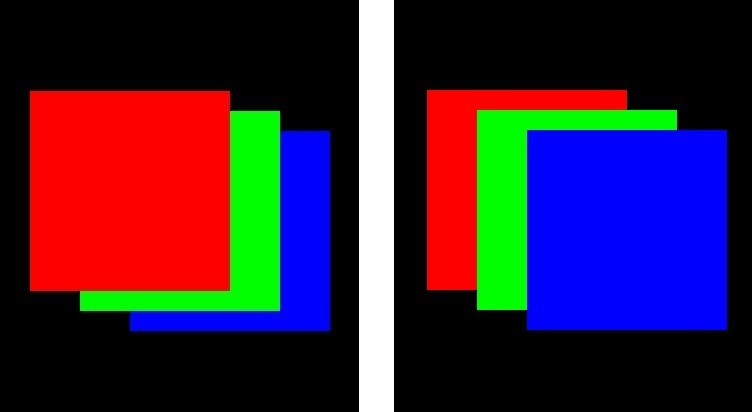
\includegraphics[scale=0.8]{images/calque-exemple}
  \caption{Exemple d'application des calques}
  \label{fig:calque-ex}
\end{figure}

La figure~\ref{fig:calque-ex} représente deux captures d'écran de marques.
Ces marques ont la même position et la même couleur dans les deux cas, mais nous avons échangé le calque 
de la marque rouge avec celui de la marque bleue dans la deuxième capture, mettant ainsi la marque bleue
au premier plan.

\subsubsection{Implémentation}

Tout d'abord, nous avons besoin d'une collection pour stocker les marques de notre calque.
Nous avons choisi de les stocker dans un vecteur pour plusieurs raisons.
La \href{https://doc.rust-lang.org/std/collections/index.html}{documentation} de Rust précise que le
vecteur et la hashmap sont à utiliser dans la plupart des cas et que ces deux collections sont très
performantes.
De plus, nous souhaitons pouvoir être capable de récupérer une marque en O(1) et ajouter une marque en
O(1) (bien que l'ajout n'est pas dans tous les cas en temps constant, par exemple dans le cas où le 
vecteur a besoin d'être réalloué pour augmenter sa taille). Ces contraintes nous confortent dans notre 
choix du vecteur.

Nous n'avons pas mentionné la suppression des marques volontairement. La raison est que nous ne supprimons
jamais de marques de nos vecteurs. La motivation derrière ce choix est que nous souhaitons une performance
maximale, ce qui implique avoir l'ajout, la récupération et la suppression en temps constant, quitte à
ce que la consommation mémoire soit importante.
Ainsi, nous avons introduit un mécanisme d'"invalidation" de marques. Lorsque l'utilisateur souhaitera
supprimer une marque et ne plus l'afficher dans sa fenêtre, \textit{contrast} invalidera la marque.
L'invalidation d'une marque indique à \textit{contrast} qu'il faudra l'ignorer lors du prochain
rafraichissement de l'écran, la faisant ainsi disparaître de la fenêtre.

Ce mécanisme seul n'est pas très intelligent car nous pourrions très vite accumuler des marques invalides
, qui ne servent à rien, dans notre vecteur.
C'est pour cette raison que nous avons introduit une pile stockant les index des marques invalides.
La pile nous permet un ajout en O(1) et c'est tout ce dont nous avons besoin pour stocker nos index.
Désormais, lors de la suppression d'une marque, nous empilons également l'index de cette marque.
Lors de l'ajout d'une marque, nous pouvons dépiler, si notre pile n'est pas vide, pour remplacer la
marque invalide à cet index par une nouvelle marque valide.

Ce mécanisme, bien que performant, complexifie légèrement l'ajout de nouvelle marque. Il ne suffit pas de
push une marque dans le vecteur, il faut d'abord vérifier s'il y a des marques invalides qui peuvent être
remplacées. 
De plus, une marque ne pouvant pas être dans deux calques à la fois, lorsque l'on souhaite ajouter une 
marque dans un calque et que celle-ci était déjà dans un autre calque, il faut nécessairement :
\begin{itemize}
\item cloner la marque de l'ancien calque
\item invalider la marque de l'ancien calque
\item ajouter correctement le clone de la marque dans le nouveau calque
\end{itemize}
Pour cloner la marque, le nouveau calque a besoin de connaître les autres calques. C'est pourquoi un 
calque a un pointeur vers \textit{contrast}. Cela permet à un calque d'accéder aux autres calques et d'en 
récupérer les  marques. C'est également la raison pour laquelle le code des calques contient une zone 
\gls{unsafe}. Nous avons besoin de déréférencer le pointeur de \textit{contrast} pour accéder aux calques et à 
leurs marques.

Nous avons également ajouté deux fonctions utilitaires permettant d'appliquer des modifications à toutes
les marques d'un calque. L'une permet de faire bouger les marques d'une certaine distance, l'autre prend 
en paramètre une fonction définie par l'utilisateur, et applique cette fonction aux marques. L'utilisateur
peut ainsi appliquer n'importe quelle modification à l'ensemble des marques d'un calque.

\subsection{Animation des marques}
\subsubsection{Qu'est-ce qu'une animation de marque ?}

Une marque animée est une marque dont le changement de propriété se fait progressivement.
Si l'on change la position d'une marque animée, on verra la marque se déplacer de manière fluide vers la
nouvelle position. Si l'on change la forme d'un marque de type point, nous verrons la transformation en la nouvelle forme progressivement.
La figure~\ref{fig:anim-ex} illustre la transformation d'une marque ayant la forme "Astérisque" vers une 
forme "Trèfle".

\begin{figure}[htp]
  \centering
  
\includegraphics[scale=0.8]{images/anim-exemple}
  \caption{Exemple d'animation pour le changement de forme}
  \label{fig:anim-ex}
\end{figure}

\subsubsection{Implémentation}

Par manque de temps, nous n'avons pas implémenté les animations en utilisant 3 buffers, comme c'était le
cas pour FATuM. Cela nous aurait demandé un changement trop important de l'architecture déjà en place.

À la place, nous avons créé une structure avec un type générique, \textit{AnimationAttribute}.
Notre structure de marque doit contenir autant d'\textit{AnimationAttribute} qu'il y a de propriétés et le
type paramamétré sera celui de la propriété.
Cette structure permet de stocker :
\begin{itemize}
\item La valeur de l'attribut qu'avait la marque avant le début de l'animation, que nous appelerons l'« 
\textit{ancienne valeur} ».
\item La valeur qu'aura l'attribut de la marque à la fin de l'animation, la « \textit{valeur cible} »
\item Le temps au moment où l'animation a commencé, le « \textit{temps de début} ».
\end{itemize}

Pour effectuer une animation d'une propriété, nous utilisons la fonction 
\textit{\href{https://www.khronos.org/registry/OpenGL-Refpages/gl4/html/mix.xhtml}{mix}} de GLSL, qui effectue une
interpolation linéaire entre deux valeurs. 
Elle prend 3 paramètres : 
\begin{itemize}
\item le début de la plage dans laquelle interpoler, « \textit{x} »
\item la fin de la plage dans laquelle interpoler, « \textit{y} »
\item la valeur à utiliser pour interpoler entre x et y, « \textit{a} ».
\end{itemize}

\textit{x} correspond à l'\textit{ancienne valeur} de la propriété et \textit{y} correspond à la 
\textit{valeur cible}.
Pour obtenir une animation propre et fluide, il faudrait que \textit{a} croisse lentement de 0 à 1.
Pour revenir à l'exemple d'animation de forme précédent, 0 correspondrait à la première marque, 0.5 
correspondrait à la troisième, et 1 correspondrait à la dernière.

Le \textit{temps de début} est récupéré grâce à un timer que nous lançons au démarrage du programme.
En passant ce timer aux shaders en tant qu'\gls{uniform}, nous sommes donc capable d'obtenir une croissance
de \textit{a} nous garantissant une animation fluide, en utilisant la formule suivante :
\textit{valeur interpolée = mix(ancienne valeur , valeur cible , min(t - temps de début , 1.0))} où t est 
le temps  écoulé depuis le lancement de l'application.
Nous utilisons la fonction minimum pour s'assurer que \textit{a} se dépasse jamais 1. Une valeur de 
\textit{a} supérieure à 1 donne lieu à des formes très étranges et fausse.

Jusqu'ici, les animations fonctionnent. Seulement, rien n'empêche l'utilisateur de modifier une propriété pendant une animation, donnant lieu à des comportements confus.
Pour cette raison, nous ignorons les modifications faites à une propriété si celle-ci est en cours
d'animation.

On notera également que cette implémentation permet d'animer plusieurs propriétés en même temps.

\subsubsection{Difficultés rencontrées}

La première difficulté a été de trouver comment implémenter les animations sans modifier l'architecture 
principale. La solution a été de modifier directement les structures des 
marques en elles-mêmes et de ne pas toucher à la structure principale. La partie précédente décrit plus en 
détails l'implémentation de cette solution.

La deuxième difficulté a été d'implémenter les animations dans \textit{contrast}.
En effet, dans un premier temps, nous les avions implémenté de manière indépendante à \textit{contrast} et avec une seule marque. Cette implémentation marchait certes correctement mais l'adapter à \textit{contrast} n'a pas été trivial.
Dans cette implémentation, nous détections la fin d'une animation de manière différente. Nous vérifions 
dans la boucle principale si l'animation était terminée pour chaque marque, et nous la mettions à jour si 
c'était le cas.
Mais imaginons cette mécanique avec plus de 200 000 marques : si elles étaient toutes animées en même 
temps, l'application ne pourrait jamais atteindre les 60 images par seconde.
Nous avons donc enlevé cette vérification quand nous avons implémenté les animations dans \textit{contrast}
pour des raisons évidentes de performances.
À la place, nous vérifions si une animation est finie seulement lorsque que l'on souhaite modifier la 
marque, donc dans les setters.

\subsection{Bibliothèques externes utilisées}

\section{Analyse du fonctionnement du logiciel}

\subsection{Ce qui fonctionne}

\subsection{Ce qui ne fonctionne pas}

\subsection{Tests et résultats}

\subsection{Benchmark}

\subsection{Les bugs}

\section{Conclusion}
%\nocite{*}
\printglossaries
\printbibliography
 
\end{document}